\documentclass[12pt,a4paper,oneside,onecolumn]{article}

\usepackage[spanish,es-noshorthands]{babel}
\usepackage{epsfig}
\usepackage[latin1]{inputenc}
\usepackage{amsmath}
\usepackage{amsfonts}
\usepackage{amssymb}
%\usepackage{mathabx}  Compila pero borra el pdf?
\usepackage{array}
\usepackage[left=1.8cm, right=1.8cm, top=2.50cm, bottom=2.5cm]{geometry}
\usepackage{hyperref}
\usepackage{color}
\usepackage{fancyhdr}
\usepackage{listings}
\usepackage{xcolor}

\pagestyle{fancy}

\fancyhead{}
\fancyfoot{}

\setlength{\headsep}{0.4cm}
\setlength{\footskip}{1.6pt}
\setlength{\parindent}{0pt}
\setlength{\extrarowheight}{1.5pt}


\lhead{An\'alisis Matem\'atico I}
\rhead{Javier Orti}
\renewcommand*\headrulewidth{0.4 pt}
\lfoot{\vspace{0.45cm}Pr\'actica 4}
\cfoot{\vspace{0.01cm}\rule{\linewidth}{0.4pt}}
\rfoot{\vspace{0.45cm} P\'ag. \thepage}

\renewcommand{\labelitemi}{$\bullet$}
\renewcommand{\labelenumi}{\theenumi)}
\renewcommand\spanishtablename{Tabla}

\decimalpoint

\headheight 16.7pt 
\textheight 715pt 

\parskip 8pt  

\hypersetup{
	colorlinks=true,
	linkcolor=blue,
	filecolor=magenta,      
	urlcolor=cyan,
}

% Python code settings
\definecolor{codegreen}{rgb}{0,0.6,0}
\definecolor{codegray}{rgb}{0.5,0.5,0.5}
\definecolor{codepurple}{rgb}{0.58,0,0.82}
\definecolor{backcolour}{rgb}{0.95,0.95,0.92}

\lstdefinestyle{mystyle}{
	backgroundcolor=\color{backcolour},   
	commentstyle=\color{codegreen},
	keywordstyle=\color{magenta},
	numberstyle=\tiny\color{codegray},
	stringstyle=\color{codepurple},
	basicstyle=\ttfamily\footnotesize,
	breakatwhitespace=false,         
	breaklines=true,                 
	captionpos=b,                    
	keepspaces=true,                 
	numbers=left,                    
	numbersep=5pt,                  
	showspaces=false,                
	showstringspaces=false,
	showtabs=false,                  
	tabsize=2
}

\lstset{style=mystyle}

\usepackage[shortlabels]{enumitem}
\usepackage{cancel}

\begin{document} 
     % Ejercicio 1 %
    \section{}
    Dividimos la integral en tres senales diferentes e integramos por separado:
    \[
    x_1(t) = \cos{(\pi t)}\delta{(t-2)}, x_2(t) = 3e^{-t}\delta{(t + 1)}, x_3(t) = \sin{(\pi t)} \delta{(2t - 1)}
    \]
    Por la propiedad selectiva de la delta sabemos que $\int_{-\infty}^{\infty}{x(t)\delta{(t-t_0)}dt = x(t_0)}$:
    \[
    I_1 = \int_{-\infty}^{\infty}{\cos{(\pi t)}\delta{(t-2)}}dt = \cos{(2\pi)} = 1
    \]
    \[
    I_2 = \int_{-\infty}^{\infty}{3e^{-t}\delta{(t + 1)}}dt = 3e
    \]
    \[
    I_3 = \int_{-\infty}^{\infty}{\sin{(\pi t)} \delta{(2t - 1)}}dt = \sin{\pi / 2} = 1
    \]
    Por tanto la integral original ser\'a:
    \[
    I = \sum_{n=1}^{3}{I_n} = 3e + 2
    \]
    
    % Ejercicio 2 %
    \section{}
     \begin{enumerate}[a)]
     \item \[
        P_\infty = \lim_{T \to \infty}{\frac{1}{2T} \int_{-T}^{T}{|x(t)|^2}dt} = \lim_{T \to \infty}{\frac{1}{2T} \int_{0}^{T}{1}dt} =
        \lim_{T \to \infty}{\frac{1}{2T}}\cdot[t]^T_0 = \frac{1}{2}
     \]
     Por tanto la primera se\~nal est\'a definida en potencia y $E_\infty = \infty$
     \item \[
        E_\infty = \int_{-\infty}^{\infty}{|e^{-at}|^2}dt =
     \]
     como $x_2(t)$ es estrictamente positiva, obviamos el valor absoluto y con la funci\'on escal\'on nos queda:
     \[
     = \int_{0}^{\infty}{e^{-2at}}dt = \frac{-1}{2a}[e^{-2at}]^\infty_0 = \frac{1}{2a}
     \]
     Por tanto la segunda se\~nal est\'a definida en energ\'ia y $P_\infty = 0$
    \end{enumerate}
    
    
    % Ejercicio 3 %
    \section{}
    Solo viendo la imagen podemos sacar la siguiente informaci\'on: $T_0 = 2\pi , w_0 = 2\pi /T_0 = 1$.\newline Por ser una funci\'on impar: $a_k = 0, c_0 = 0, x(t) = \sum_{k = 1}^{\infty}{b_k \cdot \sin{(kt)}}$ \newpage
    La se\~nal $x(t)$ es muy f\'acil de definir en el periodo que contiene a $t =0$, ya que se trada de la recta $y = t$, o lo que es lo mismo:
    \[
        x(t) = \begin{cases}
            t, & \text{ si $-\pi < t < \pi$}  \\
            ...
        \end{cases}
    \]
    Calculamos los coeficientes (Obtenemos una integral por partes sencilla):
    \[
        b_k = \frac{2}{T_0}\int_{\langle T_0 \rangle}{x(t)\sin{(k w_0 t)}}dt = \frac{1}{\pi}\int_{-\pi}^{\pi}{t\sin{(k w_0 t)}}dt = \left[\frac{-t}{\pi k}\cos{(k t)} + \frac{\sin{(k t)}}{\pi k^2}\right]^\pi_{-\pi} = \frac{-2 \cos{(\pi k)}}{k}
    \]
    Como nos piden los 5 primeros senos y cosenos, calculamos hasta k=5 sustituyendo:
    \[
        b_1 = \frac{-2}{1}\cos{(\pi)} = 2, b_2 = -1, b_3 = \frac{2}{3}, b_4 = \frac{-1}{2}, b_5 = \frac{2}{5}
    \]
    Por tanto el desarrollo de fourier resultante:
    \[
        x_5(t) = \sum_{k = 1}^{5}{b_k \cdot \sin{(kt)}} = 2\sin{(t)} -\sin{(2t)} + \frac{2}{3}\sin{(3t)} - \frac{1}{2}\sin{(4t)} + \frac{2}{5}\sin{(}
    \]
    \href{https://www.geogebra.org/calculator/btne8shm}{\underline {Animaci\'on de la serie de fourier resultante}}  (en geogebra, pulsar 'play' en la variable $k$)
    Como se ve en la gr\'afica, Se aprecia claramente el fen\'omeno de Gibbs ya que en las discontinuidades, al aproximar por Fourier, se produce un error considerable respecto a la se\~nal original.
    
     % Ejercicio 4 %
     \section{}
     Calculamos la transformada:
     \[
        X(\omega) = \int_{-\infty}^{\infty}{e^{-2(t-1)}\cdot e^{-j\omega t} \cdot u(t-1) dt} = \int_{1}^{\infty}{e^{-2(t-1)}\cdot e^{-j\omega t} dt} = \frac{1}{-2-j\omega}\left[e^{-2t+1}\cdot e^{-jt\omega} \right]^\infty_1 = 
     \]
     Como coseno y seno oscilan entre 1 y -1, resolvemos la indeterminaci\'on:
    \[
        = \frac{1}{-2-j\omega}\left[ \frac{\cos{(\omega t)} - j\sin{(\omega t)}}{e^{-2t + 1}} \right]^\infty_1 = \frac{e^{-1 -jw}}{2 + jw}
    \]
    Calculamos ahora su m\'odulo:
    \[
        |X(\omega)| = \frac{|e^{-1 -jw}|}{|2 + jw|} = \frac{e^{-1}}{\sqrt{4 + \omega ^2}}
    \]
    Desarrollamos ahora la segunda se\~nal:
    \[
        Y(\omega) = \int_{-\infty}^{\infty}{e^{-2|t-1|}\cdot e^{-j\omega t}}dt 
    \]
    Separamos en dos partes el valor absoluto: 
    \[
        Y(\omega) = \int_{-\infty}^{1}{{e^{2t-2}}\cdot e^{-j\omega t}}dt + \int_{1}^{\infty}{{e^{-2t+2}}\cdot e^{-j\omega t}}dt =
    \]
    \[
        \left [\frac{e^{2t-2-j\omega t}}{2-j\omega} \right]^{1}_{-\infty} + \left [\frac{e^{-2t+2-j\omega t}}{-2-j\omega} \right]^{\infty}_{1} = \frac{e^{-j\omega}}{2-j\omega} + \frac{e^{-j\omega}}{2+j\omega}
    \]
    Simplificamos con un denominador com\'un y simplificando:
    \[
        Y(\omega) = \frac{4e^{-j\omega}}{4+\omega ^{2}}
    \]
    Su m\'odulo:
    \[
        |Y(\omega)| = \frac{|4e^{-j\omega}|}{|4+\omega ^{2}|} = \frac{4}{4+\omega ^ 2}
    \]
    Representamos en geogebra:
    \begin{figure}[!h]
		\centering
		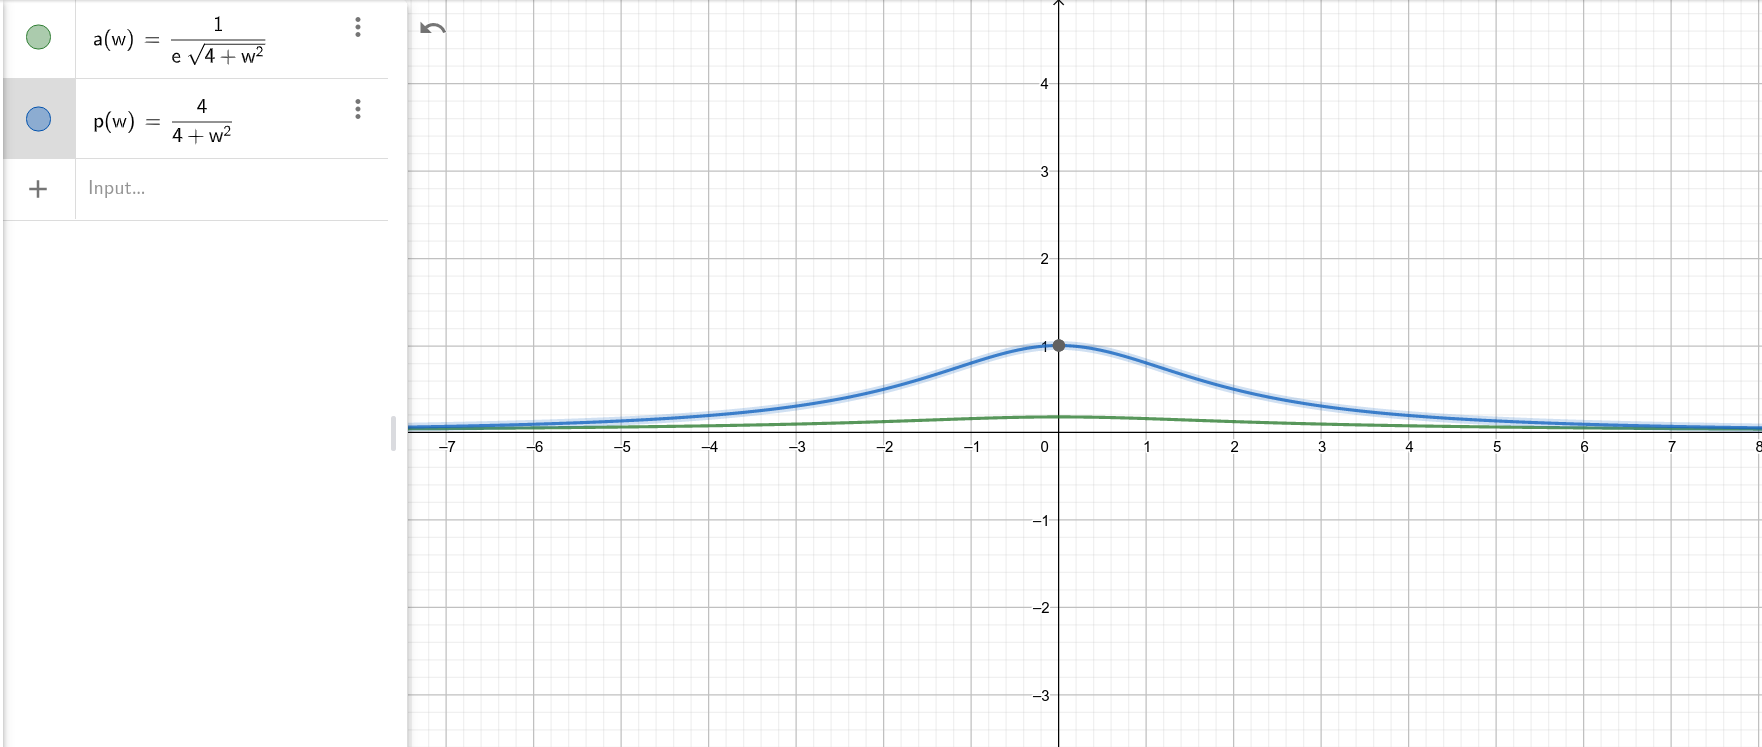
\includegraphics[scale=0.3]{campanas.png}
		\caption{}
		\label{fig:1}
	\end{figure}
	Podemos apreciar que los m\'odulos forman figuras parecidas a distribuciones normales (Campana de Gauss- t-student...), por supuesto sin cumplir sus propiedades.
	
\end{document}